\chapter{Team 3 Agent Design}\label{team_3_agent_design}

\section{The Agent}\label{sec:the_agent}
Team 3’s agent design is based on the Theory of Reasoned Action (TRA) and its extension, the Theory of Planned Behaviour (TPB). The agents are designed to have a shiftable personality dependent on the three variables in Figure \ref{fig:TRA-diagram} that TPB  \cite{AJZEN1991179} links to the behaviours of an agent. These three variables, together with a social network, define its personality as a whole, \cite{victor} and influence the actions it will take.

\begin{figure}[htb]
    \centering
    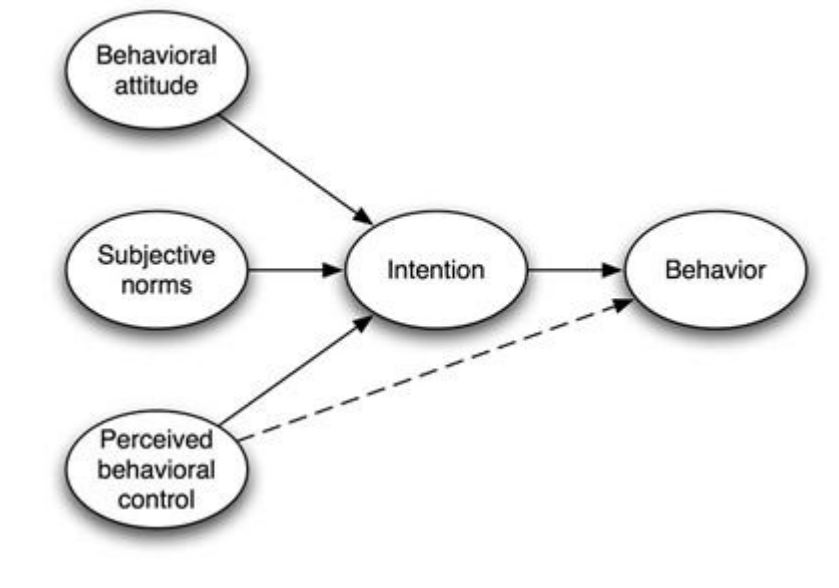
\includegraphics[width=0.5\linewidth]{005_team_3_agent_design/images/image1.jpg}
    \caption{TRA explanation.}
    \label{fig:TRA-diagram}
\end{figure}

The Theory of Reasoned Action was developed by Martin Fishbein in 1967 and was later improved by Icek Ajzen and Martin in 1980, with the Theory of Planned Behaviour. The TPB states that the behavioural intentions of individuals can be attributed to three interdependent factors: perceived behaviour control, the subjective norm, and the attitude of the individual, as shown in Figure \ref{fig:TRA-diagram}. It must be noted that the TPB is unable to accurately and consistently predict non-volitional behaviours of the individual. Therefore, TPB can only be applied to those actions for which a reason can be found. These are actions that occur as a reaction to others and that the individual has control over \cite{TRA}. This theory is applicable to agent decisions in the tower since the agent must make decisions in a reactionary manner, based on interactions with other agents.\par 
In order to apply the TPB to the agents, we define three agent variables, each corresponding to one of the three components of the theory. Using this approach, we have defined the agent variables to be: 
\begin{enumerate}
    \item \textbf{Stubbornness}: it addresses perceived behaviour control, which is the influence that external agents have on the decisions that are to be taken.
    \item \textbf{Morality}: it addresses the subjective norm, which is one's idea of what is socially perceived to be right or wrong.
    \item \textbf{Mood}: it defines the attitude towards the action to take.
\end{enumerate}
These variables are modified as an agent interacts, which leads to our agent having mutable behavioural intentions, and making decisions with different “intended outcomes” as the variables change. \par
In literature surrounding the substantive uniqueness of human behaviour \cite{TRA} Martin Fishbein argues that no two agents will react identically to the same circumstances. In practice, reactions tend to be normally distributed, with a random aspect to them. To account for this, all possible changes to internal agent variables are implemented by specifying the range within which the variable can change. The final change to the variable is randomly selected from within this range. This characteristic of randomness in the agents’ behaviour compensates for the fact that the TPB does not take into account non-volitional behaviours, so including this randomness makes the agent act in a more human-like manner.\par 
The next step after identifying the agent strategy was to think about the scenario and how the problem should be solved. Our first approach used classical game theory, which states that under normal circumstances, an unbiased agent would always prioritise themselves and their needs over anything else. Hence, this dictates that each agent should not act in a moral way at all. In our scenario, this leads to agents taking very large amounts of food, causing agents below them to have access to less food, and have a greater likelihood of death. However, we found research demonstrating how humans in a social environment tend to make decisions benefiting the collective \cite{batson_batson_todd_brummett_shaw_aldeguer_1995}. This contradicted traditional game theory views and made this approach unreasonable when trying to recreate a human type behaviour, following the two most common explanations of why humans violate classic game theory: enlightened self-interest and group identity.\par 
Enlightened self-interest includes a human’s awareness of long-term consequences, along with their desire to avoid social punishment and self-punishment. Assuming a group identity is the act of regarding the goals of the collective as one's own goals. In the tower, agents with a group identity would see their own primary purpose as ensuring that all agents in the tower survive, and not that it has survived as an individual. As such, it feels like its social network is an extension of itself and care for it greatly. According to research, the above factors are sufficient to make humans behave in a different manner within a collective than classic game theory would dictate.\par
With this in mind, we further extended our definition of the agent variables and changed the way our agent would use them. In addition, we implemented a social network by defining an additional “friendship” variable, to aid the agent in assuming the aforementioned group identity.\par 
\begin{enumerate}
    \item \textbf{Stubbornness}: Defines the willingness of the agent to read the messages it receives, and in doing so, form relationships. Due to this, it is also more or less willing to succumb to peer pressure. In general, stubbornness can be summarised as the willingness to change views based on possible long-term consequences. This is reflected in how the agent reacts to different messages, on the basis of enlightened self-interest and not wanting to be punished for their behaviour.
    \item \textbf{Mood}: An agent’s willingness to consider the group identity at a given time. The agent’s decisions will benefit the group more the better the mood they are in. In the tower this is translated as eating less food when possible, aiming for the preservation of the group. 
    \item \textbf{Friendship}: The degree to which another agent believes an agent has acted in its own self-interest. This defines the degree of social punishment or praise that an agent receives. This will naturally divide an agent’s perspective of other agents into those who act in their own self-interest and those who do not. The agent interacts with these two perceived categories of agent differently.
    \item \textbf{Morality}: A measure of susceptibleness to guilt, which is a form of self-punishment. On top of this, morality also represents the degree to which agents are conscious of the group identity. Knowing that other agents are suffering or dying, especially ones that belong to the agent's social network, will make the agent feel guilty and more willing to help others if their morality is high. 
\end{enumerate}
The agent will interact and make decisions based on a combination of these variables, as defined above. More information is given in the sections below, which explains different aspects of the agent, such as their daily actions, memory, decision taking and communication. 

\subsection{Action Process}
The Agent takes the following steps during their day: 
\begin{enumerate}
    \item The agent starts by updating its defining variables at the beginning of each day based on their HP. This acts as the agents checking in on itself and changing its attitude(mood) and morality depending on its condition(HP). 
    \item If the agent was just ‘born’ it will estimate an initial value for the average food consumed based on the amount of food required to maintain, 50 health.
    \item When the tower reshuffles the agents (which each agent knows by checking what floor it is on) mood changes depending on the relative position of the new floor to the prior floor.  
    \item The agent attempts to eat every day. The quantity depends on treaties, the messages it has received and whether other agents have requested it to leave or eat a certain amount of food or a calculation based on the agent’s current values. More information on this can be found in \Cref{sec:food_intake}. 
    \item Finally, the agent will attempt to communicate with other agents and create a social network via message sending and treaty proposition. More information on this is can be found in \Cref{sec:agent_communication}. 
  \end{enumerate}

\subsection{Agent Knowledge}
Agent 3 will be able to make decisions when receiving messages or after signing treaties and remember these until it eats. This information is used to show that a predetermined decision has been taken instead of “impulsively” eating food depending solely on the agent’s hunger and state of mind. The decisions that the agent takes include:
\begin{enumerate}
    \item The floors the agent has been in before. This information will affect the agent’s mood after being reshuffled, as it would remember where they have been and know if the new floor is a good or bad one.  
    \item The last recorded HP value. Used to see changes to the agent's health.
    \item The agent’s friendship network. It is aware of the people it has met during their time in the tower. The agent’s friends are identified and are considered more or less close to the agent with an affection parameter that ranges from 0 to 1, with 0  representing a complete dislike for the other agent.
    \item The amount of food last eaten.
    \item The amount of food last seen on the platform.
    \item A moving average of food consumed.
    \item The age of the agent.
    \item The treaty we have proposed until it is accepted or rejected.
    \item The estimation of the reshuffle period.
    \item The HP our neighbour above last told us it had.
    \item The HP our neighbour below last told us it had.
\end{enumerate}

\subsection{Agent Generation}
The defining variables of the agents are randomised when it is generated in order to avoid preconditioned agents and mimic different personalities. All three variables are defined to be in the range 0 to 100. Morality and mood are randomly allocated to a value in the range, but stubbornness is limited to a number between 0 and 75. As explained in our agent parameters, stubbornness represents the effect of external influences on an agent. A stubbornness of 100 would mean this agent is completely unwilling to listen and would ignore all incoming messages, effectively making them an agent that disrupts the tower. In order for this to not be the case, we added the artificial upper bound to the value of stubbornness.\par 
As Shao et al. have shown in “Beyond Moral Reasoning: A Review of Moral Identity Research and Its Implications for Business Ethics” \cite{shao_aquino_freeman_2008}, one’s moral action is most heavily influenced by their moral personality, as opposed to their moral reasoning, which empirically seems to show only a minor influence on the moral behaviour of an agent \cite{blasi_1983}. Hence, we used the variance and unpredictability to initialise our agents randomly on the moral scale. This insight also allowed us to witness a purely emergent strategy and nature as opposed to a pre-programmed inherent morality.\par 
While the implementation of initial randomness alone allowed for interesting strategies to occur, we also wanted the agents to adapt their morality on the basis of their community and associations, as argued by Shao. This was made possible by having all actions an agent does affect its emotion variables. \par 

\section{Agent Communication}\label{sec:agent_communication}
Communication between agents is fundamental for the possibility of collaboration and self-organisation between agents. Crowd behaviour is considered to be generated by individuals, context-dependent and dynamic, as defended by the modern foundation of crowd behaviour \cite{0d9bc1ee81234780b2bb6ecd02762d56}. In this project, communication between agents is based on two concepts, treaties and direct messages, which are equally exploited by the Team 3 agent and combined with the conceptualization of friendship levels. 

\subsection{The Agent’s Social Network}
The agent forms relationships with others surrounding it as they communicate with each other. The agent remembers everyone it has met and assigns a level of friendship to them depending on their interactions. By doing this, the agent forms a social network that will affect its decisions, something that the Theory of Planned Behaviour explores in the “subjective norm” aspect of the theory. In the TPB,  all three main variables are interdependent and for this reason, the agent will have a better or worse opinion of someone it has just met depending on their morality at that point. \par
The large importance which the agent places on friendship is not only a logical interpretation of the TPB. In fact, it is a notion which philosophers and legislators have repeatedly confirmed throughout the ages. For example, the Aristotelian concept of friendship defends it as “the finest way we exercise practical reasoning”. Quoting Aristotle: “Friendship seems to hold cities together, and lawgivers seem to care for it more than for justice … and when men are friends, they have no need for justice”, friendship is considered the best form of human moral action by The Nicomachean Ethics \cite{sokolowski}. Thus, it is no surprise that friendship is fundamental in the decision-making process of the agent, and also in its responses to communication initiated by other agents. \par 
To provide an alternative perspective on friendship, McCullough et al. investigate the nature of prosocial action and gratitude’s place in transactions \cite{doi:10.1111/j.1467-8721.2008.00590.x}. The friendship function allows the agent to assign a level of gratitude in response to the prosocial action of the other agents. In this way, the agent could more effectively alert themselves to the prosocial nature of another’s actions. By utilising the friendship function to, in turn, behave more prosocially to those who have done so to us, we embedded a system of gratitude in the agents’ actions. This allows the agents to be more capable of self-organising.\par 
We further developed the agent's response to actions taken by foreign agents by evaluating the selflessness of the action taken. That is to say, the more severe the sacrifice another agent makes, the more grateful the agent becomes. This is based on McCullough’s definition that one experiences gratitude when “they have benefited from someone’s costly, intentional, voluntary effort on their behalf”. \par 
Emotions allow us to respond to reality in a self-protective and self-enhancing way \cite{ekman_1992}, it was this response that we wanted the agent to embody so that emotions could govern the evolution of their actions, by either leading them on a self-protective path, if circumstances caused selfish agents to prevail, or a self-enhancing manner, as cooperation would beget further cooperation through the agents' system of gratitude.\par
This is the basis of our friendship metric and implies the agent will react more positively to a friend and will increase the friendship of those with whom it has positive interactions.

\subsection{Message Sending}
Message sending is determined by a probabilistic decision, with each message having a 20 percent chance of being sent. The direction the messages are sent in is determined by the moral state of the agent. When the agent's morality is low, they will tend towards self-preservation and send messages upwards requesting information or help. On the other hand, when morality is high, the agent will look to create a stable society as stated by their willingness to look ahead and communicate with those below them to offer help and information, aiming to fortify their social network.\par 
The design of message passing has various noteworthy characteristics that act to aid the agent fulfil its intentions:
\begin{enumerate}
    \item The agent prioritises itself when its HP is critical, opting for treaties and messages that involve other agents leaving food in the platform and utilising this mechanic as a failsafe when in danger.
    \item The agents take into account the neighbours' health when sending messages proposing how much food to leave on the platform. This makes the message more likely to be accepted. 
\end{enumerate}

\subsection{Message Reception}
When messages are involved, stubbornness is used to decide to ignore or read a message, with its reaction or answer also being dependent on the stubbornness of the agent. \par
The agent will follow the next process when a message is received:
\begin{enumerate}
    \item The agent will decide to ignore or read the message, with a probability of ignoring the message equal to the stubbornness level.
    \item If the agent decides to read the message it is analysed and matched with the type of response or responses acceptable for the message. 
    \item The agent will note the agent that sent the message and consider the friendship level it shares with the sender. Friendship together with the morality level and the content of the message itself will decide the exact content of the response.
    \item The content of the message and its sender will affect the agents’ emotional variables and the friendship level with the sender. This change affects the future reaction to communication done by other agents and the decisions taken by the agent from that point onwards. 
\end{enumerate}
To ensure a minimum level of communication all messages read will be answered by the agent. 

\subsection{Reaction to Received Messages}
The changes are dependent on four criteria to determine initial agent characteristic manipulation. These four variables are the variables present upon the receipt of the message and somewhat representative of the type 1 brain system discussed in \cite{kahneman_tversky_2000}, \cite{frankish_2010}. \par
The initial emotional response is based on the variables of the immediate past, the hp moving average on the last five ticks, opposed to the overall hp average, or welfare average. This is to represent the subconscious layer of emotional response, as seen in \cite{kamble_2021}, whereby our response to the situation is more irrational and illogical than the conscious mind perceives. \par
Summing the net total of all the initial responses to zero, allows us to explore the oscillatory nature of emotion while avoiding the possible pitfall of any dominant emotions. \par
\begin{table}[htb]
    \centering
    \begin{tabular}{@{}lllll@{}}
    \toprule
    HP dec last tick [nonfriend]    & Stubbornness      & Morality         & Mood             & Friendship     \\ \midrule
    ask Food Taken                  & 0                 & -0.5             & -0.5             & 0              \\
    ask HP                          & 0                 & -0.5             & -0.5             & 0              \\
    ask Intended Food Intake        & 0                 & 0                & 0                & 0              \\
    Request Take Food               & 1                 & -0.5             & -1               & -1             \\
    Request Leave Food              & 1                 & -0.5             & -1               & 0              \\ \bottomrule
    \end{tabular}
\end{table}
\begin{table}[htb]
    \centering
    \begin{tabular}{@{}lllll@{}}
    \toprule
    HP inc last tick [nonfriend]    & Stubbornness      & Morality         & Mood             & Friendship     \\ \midrule
    ask Food Taken                  & 0                 & 0                & 0                & -1             \\
    ask HP                          & -1                & 1                & 1.5              & 1              \\
    ask Intended Food Intake        & 0                 & 0                & 0                & 0              \\
    Request Take Food               & 0                 & 0                & 0                & 0              \\
    Request Leave Food              & -1                & 1                & 1.5              & 1              \\ \bottomrule
    \end{tabular}
\end{table}
\begin{table}[htb]
    \centering
    \begin{tabular}{@{}lllll@{}}
    \toprule
    Sum total                       & Stubbornness      & Morality         & Mood             & Friendship     \\ \midrule
    Request Leave Food              & 0                 & 0                & 0                & 0              \\ \bottomrule
    \end{tabular}
    \caption{Message Reactions.}
\end{table}
This zero-sum agent is how the agent is currently set, it represents the neutral agent. One who possesses no inherent emotional bias. This was done by balancing the positive and negative reactions to a friend, and those to a non-friend separately. We noticed the need for this when the agent would initially get stuck at the positive and negative limits of certain emotions. As future work, it would be exciting to see the emergent strategies which we hope to observe as we introduce biases. For instance, an agent whose net sum of all interactions leaves them with a stubbornness increase, coupled with an inherently moral agent, may create strategies yet thought of. 

\subsection{Proposing a Treaty}
When the agent HP is critical, it will ask for help by either asking for the agent above to leave at least the amount of food necessary to survive or, if it doesn’t have any active treaties, a treaty that states: if HP is higher than 20 leave 95\% of the food in the platform for 3 days. At this time the agent's self-preservation instinct takes precedence and its objective becomes to eat enough food to get out of the critical state before the agent dies.
When the agent is not in critical condition, it is able to propose other treaties depending on their morality. The first treaty is detrimental for the tower and the other two are ‘fair’ treaties for the tower. \par
\begin{enumerate}
    \item If the agent is very immoral, it will send a treaty that is detrimental for anyone above them. It is expected for this treaty to be rejected by any sensible agents and is done as a way of mimicking frustration or the desire to hurt others when morality is low.
    \item If HP is below 60 leave at least 60\% of the food on the platform for 5 days. This treaty tries to encourage immoral agents in higher positions to share food. 
    \item If HP is below 10 leave at least 95\% of the food on the platform for 10 days. This treaty is aimed at moral agents that would be willing to start eating less until it is close to death.
\end{enumerate}
Both of the last treaties are proposed randomly by the agent, without a specific proclivity for any of the two. The randomness of the treaty selection is done to increase the volitional behaviour of the agent. Characteristics that the agent inherently lacks if its personality is solely based on the TRA.

\subsection{Handling a Proposed Treaty}
In our strategy, we have decided to perform complex evaluation of food treaties. To evaluate how risky a treaty is, the two key metrics that are included in treaties will be used. These are the minimum agent condition at which the treaty is activated, and the maximum food that the treaty allows an agent to take.\par
Agents that are in a bad mood will not accept treaties that it needs to honour when it is in very low health, since it  has low confidence in the capabilities of other agents. However, when in a good mood agents will accept treaties that must be honoured even at low health. Morality is an indicator of the agent’s desire to perform actions that will benefit others, as opposed to just benefiting the agent itself. Therefore, very moral agents will accept treaties that involve consuming just enough food to survive, but not too little food that it dies or too much that it is too greedy. Similarly, very immoral agents will only accept treaties where it consumes more than enough food since it disregards the food needs of the other agents. The table below displays the mood and morality values that agents must satisfy to accept treaties with any given condition depending on the agent’s health, and the food the agent would have to leave according to the request of the treaty.

\begin{table}[htb]
    \centering
    \resizebox{\textwidth}{!}{\begin{tabular}{|l|l|l|l|l|l|l|l|}
    \hline
        mood (m)/morality (M)   & ~                                     & 0 $<$ morality $<$ 40     & 20 $<$ morality $<$ 60    & 40 $<$ morality $<$ 80    & 60 $<$ morality $<$ 100   & morality $>$ 80       & morality $>$ 100      \\ \hline
        ~                       & AgentPosition $\backslash$ FoodTaken  & VeryLarge (1)             & Large (2)                 & Moderate (3)              & Little (4)                & SurvivalAmount (5)    & TooLittle (6)         \\ \hline
        mood $>$ 0              & Strong (1)                            & m$>$0, 0$<$M$<$40         & m$>$0, 20$<$M$<$60        & m$>$0, 40$<$M$<$80        & m$>$0, 60$<$M$<$100       & m$>$0, 80$<$M         & N/A since 100$<$M     \\ \hline
        mood $>$ 20             & Healthy (2)                           & m$>$20, 0$<$M$<$40        & m$>$20, 20$<$M$<$60       & m$>$20, 40$<$M$<$80       & m$>$20, 60$<$M$<$100      & m$>$20, 80$<$M        & N/A since 100$<$M     \\ \hline
        mood $>$ 40             & Average (3)                           & m$>$40, 0$<$M$<$40        & m$>$40, 20$<$M$<$60       & m$>$40, 40$<$M$<$80       & m$>$40, 60$<$M$<$100      & m$>$40, 80$<$M        & N/A since 100$<$M     \\ \hline
        mood $>$ 60             & Weak (4)                              & m$>$60, 0$<$M$<$40        & m$>$60, 20$<$M$<$60       & m$>$60, 40$<$M$<$80       & m$>$60, 60$<$M$<$100      & m$>$60, 80$<$M        & N/A since 100$<$M     \\ \hline
        mood $>$ 80             & SurvivalLevel (5)                     & m$>$80, 0$<$M$<$40        & m$>$80, 20$<$M$<$60       & m$>$80, 40$<$M$<$80       & m$>$80, 60$<$M$<$100      & m$>$80, 80$<$M        & N/A since 100$<$M     \\ \hline
    \end{tabular}}
    \caption{Treaty Acceptance.}
\end{table}

Treaties also have a specified duration and signature count, which are visible to any agent that wishes to sign the treaty. These are likely to affect an agent’s decision to accept a treaty and have been taken into account. If a treaty lasts longer than twice the reshuffle period, an agent deems it too far into the future to be able to predict what will happen and plans to reject the treaty. However, if a treaty has more than five signatures, we deem it to be a popular treaty. If the agent plans to reject the treaty as a result of any previous logic, the influence of peer pressure will cause the agent to reconsider accepting the treaty. Peer pressure is based on the concept of crowd suggestibility coined by Park, R. E.  in 1904 in his “Masse und Publikum”, \cite{Solr-413687}. The stubbornness of an agent is used as the likelihood to give in to peer pressure, so more stubborn agents are less likely to reconsider their response, and more likely to stick with their original decision.

\section{Food Intake}\label{sec:food_intake}
When taking food, an agent considers, in order of importance:
\begin{enumerate}
    \item The treaties that it has agreed to. These must be adhered to if the agent fulfils the condition specified in the treaty, and define the amount of food that the agent must leave. 
    \item Food information from the message pipeline. This can be either an amount of food that the agent must eat, or an amount it must leave, neither, or both.
    \item The health level and morality of the agent. These are used to calculate the food the agent will eat, alongside any values which have been specified in treaties or the message pipeline.
\end{enumerate}
The agent calculates the amount of food it decides to take in the following manner: 
\begin{enumerate}
    \item If the agent is not at critical health, a target HP is calculated, which is designed to make an agent's HP converge to 65 if run repeatedly. The food required to reach the target HP level is then calculated, and scaled up if the agent is immoral, or down if the agent is moral.
    \item If the agent is at critical health, the agent aims to escape this state by targeting the weak level HP. The morality of the agent will dictate if it takes just the food it needs from the platform, or more, or maybe even less. However, on the last day before an agent’s death, it must desire to take at least survival food from the platform. This logic is expressed in the diagram \ref{fig:food-diagram}.
\end{enumerate}

\begin{figure}[htb]
    \centering
    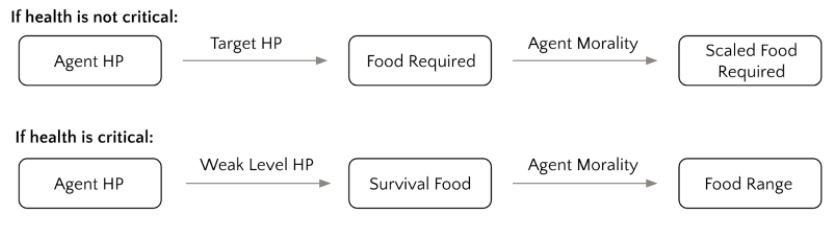
\includegraphics[width=0.85\linewidth]{005_team_3_agent_design/images/diagram1.jpg}
    \caption{Food calculation process.}
    \label{fig:food-diagram}
\end{figure}

To be more specific, an agents’ decision regarding how much food to eat and leave will fall into one of four possible categories:

\begin{enumerate}
    \item If it has decided how much food to eat and leave and both conditions can be met the agent will eat. If meeting both conditions is impossible, there is not enough food on the platform, a decision that fulfils the value of how much food to leave will be taken, with the value of how much the agent eats ranging from all that it can to just what it needs to survive. 
    \item If the agent knows how much it wants to eat but not how much to leave it will attempt to eat the amount it has decided it wants.
    \item If the agent has not decided how much to eat but knows how much to leave it will eat depending on its health condition. If its health is critical or about to die it will eat whatever it needs to survive. If its health is not of concern it will eat as much as it can while leaving the amount it has decided to leave. Morality is used to scale how much food to eat.
    \item If it is unaware of how much to leave or eat its decision will depend on its health level. If its health is critical or about to die it will eat whatever it needs to survive. If its health is not of concern, eat an amount of food scaled by its morality.
\end{enumerate}

\section{Results}
\begin{table}[htb]
    \centering
    \begin{tabular}{@{}lllll@{}}
    \toprule
        ~                       & Random Agents         & Selfish Agents         & Team 3                \\ \hline
        Deaths                  & 309                   & 322                    & 139                   \\ \hline
        Utility                 & 0.009                 & 0.013                  & 0.034                 \\ \hline
    \end{tabular}
    \caption{Experimental results.}
    \label{tab:InitalResults}
\end{table}

These experiments were run for 500 days, with 50 food for 10 agents and a reshuffle period of 7 days. Each experiment was run three times and the average taken. This means there was enough food for every agent to survive at critical level but not enough to keep them all out of critical condition. For this reason, agents need to communicate and self organise in order to decrease the amount of deaths in this strenuous circumstances.

As shown in Table \ref{tab:InitalResults}, the results indicate that the agents are capable of significantly reducing their deaths compared to random agents. This difference arises due to the Team 3 agents’ increased communication capabilities via treaties and messages, allowing them to assume a group identity. Random agents take an approach which more closely embodies the selfish approach dictated by classical game theory. As is expected, this is outperformed by a higher degree of organisation in a collective, which successfully models group identity and collective human survival instinct.

Figure \ref{fig:AvgDeaths} further shows how, even as the food in the platform changes, the Team 3 agent always outperforms the selfish and random agents.

\begin{figure}[htb]
    \centering
    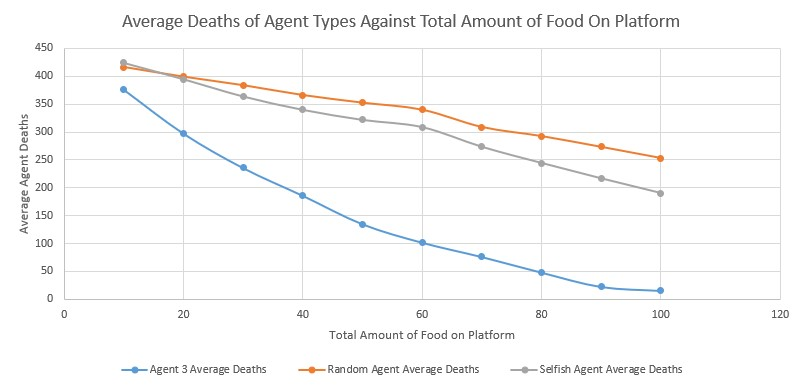
\includegraphics[width=0.9\linewidth]{005_team_3_agent_design/images/Average_Deaths_of_Agents_Against_Total_Amount_of_Food_On_Platform.jpg}
    \caption{Average deaths of agents against total amount of food on platform.}
    \label{fig:AvgDeaths}
\end{figure}

In addition, we ran tests where the Team 3 agent was placed into the tower along with another teams’ agent. Five agents from Team 3 and five from the respective team in Figure \ref{fig:AgainstOtherTeams} were simulated for 500 days and 100 total food on the platform. In Figure \ref{fig:AgainstOtherTeams} you can see the cumulative deaths of both agent types.  

\begin{figure}[htb]
    \centering
    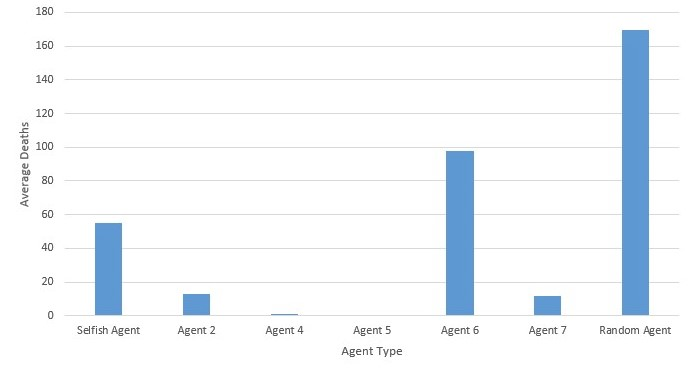
\includegraphics[width=0.8\linewidth]{005_team_3_agent_design/images/Average_Deaths_When_Cooperating_With_Another_Agent_Type.jpg}
    \caption{Average deaths when cooperating with another agent type.}
    \label{fig:AgainstOtherTeams}
\end{figure}

This indicates that Team 3 agents work best with agents from Teams 5, 4, 2 and 7. Successful cooperation with multiple other agent types demonstrates the agent’s ability to adapt to different situations and work well with agents that are also capable of assuming a group identity, and creating a self-organising structure. This point is also illustrated by examining the large number of total deaths in a tower with random agents. Their ignorant and  unpredictable actions means that the Team 3 agents cannot adapt to their behaviour or form meaningful connections with them. Hence, the system cannot evolve, causing the deaths per time period to remain relatively constant, and the cumulative deaths to be high.

Finally, we wanted to observe if the total number of agents in the tower had an effect on the outcome of the simulation, and whether fewer agents were able to communicate more effectively. This seemed to be the case, as proven by Figure \ref{fig:DeathsNoAgents}. The lower the total number of agents, the more meaningful connections they can make and the stronger the social network. This is reflected in the two-agent tower experiment, in which they successfully assumed a group identity with no deaths. This occurs because both agents agree to leave each other enough food to survive. The greater the number of agents that are in the tower, the harder it is for them to form a self-preserving social network. In this case, the importance that the agents place on the collective identity does not outweigh their desire to form instinctive, self-preservative characteristics.  

\begin{figure}[htb]
    \centering
    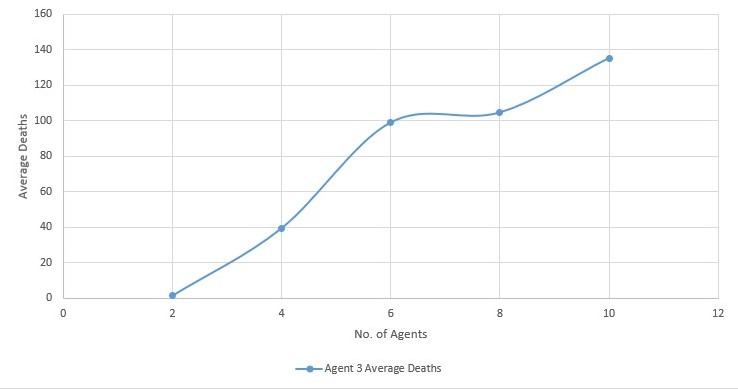
\includegraphics[width=0.9\linewidth]{005_team_3_agent_design/images/Average_Deaths_Against_No._of_Agents_With_5_Food_Per_Agent_No_Title.jpg}
    \caption{Average Deaths Against No. of Agents}
    \label{fig:DeathsNoAgents}
\end{figure}


